\chapter{Arsitektur Continer (Container Architecture)}
\authors{Richwen Canady, Desfantio Wuidjaja, Vincenzo Matalino}

\section{Latar Belakang}
Konsep container berasal dari teknologi chroot pada sistem operasi UNIX. Teknologi ini memungkinkan pengguna untuk membuat lingkungan kerja yang terisolasi pada sistem operasi UNIX. Di lingkungan kerja ini, pengguna dapat menjalankan aplikasi secara mandiri tanpa terpengaruh oleh aplikasi lain yang berjalan di sistem yang sama. Namun, teknologi chroot memiliki beberapa keterbatasan, seperti pengguna harus mengkonfigurasi secara manual, tidak mendukung manajemen sumber daya.\\
 
Pada tahun 2008, LXC (Linux Containers) mengembangkan teknologi container sebagai solusi untuk mengatasi keterbatasan teknologi chroot pada sistem operasi UNIX. Teknologi container memungkinkan pengguna untuk menjalankan aplikasi secara otomatis dan efisien dalam lingkungan terisolasi yang mudah dikelola. Teknologi kontainer berjalan di sistem operasi Linux, menggunakan kernel yang sama untuk menjalankan aplikasi di dalam container.\\

Pada 2013, Docker dirilis sebagai implementasi teknologi container yang lebih ramah pengguna dan mudah digunakan. Docker menyediakan gambar yang berisi semua elemen yang diperlukan untuk menjalankan aplikasi dalam container, termasuk aplikasi, sistem operasi, dan dependensi. Gambar Docker mudah dibuat, dikelola, dan dibagikan, dan dapat digunakan untuk penerapan cepat di lingkungan produksi.\\

Container menjadi lebih populer dan banyak digunakan untuk pengembangan dan pengelolaan aplikasi di lingkungan cloud. Container memungkinkan pengguna mengoptimalkan penggunaan sumber daya, meningkatkan portabilitas, dan mengelola aplikasi dengan mudah. Container juga mendukung orkestrasi, seperti Kubernetes, untuk mengelola aplikasi di lingkungan yang lebih kompleks. Saat ini, container adalah teknologi penting dalam pengembangan dan manajemen aplikasi.
\subsection{Virtualization vs Container Architecture}
\textit{Container architecture} dan \textit{virtualization} adalah dua teknologi yang sering digunakan dalam pengembangan dan pengelolaan aplikasi, namun ada beberapa perbedaan antara keduanya yaitu:
\begin{itemize}
	\item Isolasi= Arsitektur container menggunakan teknologi yang lebih ringan untuk menjalankan aplikasi di lingkungan yang terisolasi. Virtualisasi, di sisi lain, menggunakan teknologi hypervisor untuk mengisolasi lingkungan virtual dari sistem host. Oleh karena itu, arsitektur container lebih efisien daripada virtualisasi dalam hal penggunaan sumber daya.
	\item Sistem operasi= Arsitektur container menggunakan kernel yang sama dengan sistem operasi host untuk menjalankan aplikasi dalam container. Virtualisasi, di sisi lain, memungkinkan pengguna untuk menjalankan sistem operasi yang berbeda dalam lingkungan virtual.
	\item Portabilitas= Arsitektur container mendukung portabilitas. Pengguna dapat mengembangkan aplikasi di lingkungan pengembangan dan dengan mudah menjalankannya di lingkungan produksi. Pada saat yang sama, virtualisasi memerlukan konfigurasi yang lebih kompleks untuk menjalankan lingkungan virtual di lingkungan produksi yang berbeda.
	\item Overhead= Overhead arsitektur container lebih rendah daripada virtualisasi karena tidak memerlukan overhead hypervisor dan kernel. Oleh karena itu, arsitektur container lebih efisien dalam hal penggunaan sumber daya.
	\item Orkestrasi= Arsitektur container memungkinkan pengguna menggunakan orkestrasi (seperti Kubernetes) untuk mengelola aplikasi di lingkungan yang lebih kompleks. Virtualisasi tidak memiliki dukungan orkestrasi yang sama.
\end{itemize}

\section{Definisi Container dan Istilah-Istilah}
\textbf{Container} adalah metode menjalankan aplikasi yang memungkinkannya berjalan secara konsisten di berbagai lingkungan komputasi.\\ 
Secara sederhana, container dapat dianggap sebagai paket yang berisi semua elemen yang diperlukan untuk menjalankan aplikasi tertentu, termasuk perangkat lunak, pustaka, konfigurasi, dan ketergantungan lainnya. 

\textbf{Docker} adalah platform open source untuk mengembangkan, menguji, dan mengimplementasikan aplikasi dalam container. 
Dalam konteks Docker, container adalah lingkungan terisolasi yang dapat berjalan di host yang sama tanpa pengaruh aplikasi atau sistem operasi lain yang berjalan di host yang sama. Container dapat dianggap sebagai paket yang berisi semua elemen yang diperlukan untuk menjalankan aplikasi tertentu, termasuk perangkat lunak, pustaka, konfigurasi, dan dependensi lainnya.

\textbf{Kubernetes} adalah platform open source untuk mengelola aplikasi dalam container yang dibuat oleh Google. Kubernetes memungkinkan pengguna untuk menjalankan, mengelola, dan mengotomatiskan penerapan aplikasi dalam container secara efisien.

\textbf{Container Architecture} merupakan sebuah konsep arsitektur yang dirancang untuk menjalankan aplikasi dalam container. Container Architecture memiliki beberapa tugas yaitu Isolasi, Portabilitas, Efisiensi, Deployment.

\begin{figure}[h]
    \centering
    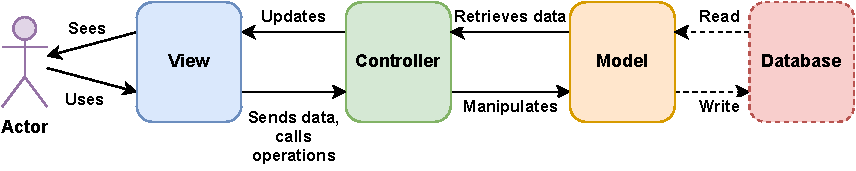
\includegraphics[width=\textwidth]{mvc}
    \caption{Arsitektur Container.}
    \label{fig:mvc}
\end{figure}

\section{Kelebihan dan Kekurangan}
Berikut adalah kelebihan dan kekurangan arsitektur MVC:


\subsection{Kelebihan}
Keuntungan dari menerapkan arsitektur MVC adalah:
\begin{itemize}
\item Pemisahan presentasi dan data membolehkan model ditampilkan di banyak \textit{view} secara bersamaan.
\item View bersifat \textit{composable} artinya view dapat dibangun dari berbagai atau berisi \textit{subviews}/\textit{fragments}.
\item Controller satu dapat diganti (\textit{switchable}) dengan controller lain pada saat \textit{runtime}.
\item Developer dapat membuat berbagai macam mekanisme pemrosesan data dari input ke output dengan mengkombinasikan berbagai macam fungsionalitas yang dimiliki oleh views, controllers, dan models.
\item \textit{Data engineers}, \textit{backend} dan \textit{frontend developers} masing-masing dapat fokus mengerjakan tugas utama mereka. 
Misal, \textit{data engineers} hanya mengerjakan tugas yang berkaitan dengan data, sendangkan \textit{frontend developers} fokus ke \textit{user interface}.
\end{itemize}

\subsection{Kekurangan}
Konsekuensi dari penerapan arsitektur MVC adalah sebagai berikut:
\begin{itemize}
\item Derajat kompleksitas kode program bertambah karena kode harus dibagi ke dalam tiga abstraksi yang berbeda.
\item \textit{Developers} harus mengikuti aturan ketat tertentu dalam mendefinisikan \textit{controllers}, \textit{models}, dan \textit{views}. 
\item Secara relative, MVC lebih sulit dipahami dikarenakan struktur bawaannya.
\item Terlalu berlebihan (\textit{overkill}) untuk aplikasi sederhana.
\item Cocok untuk pembangunan Graphical User Interface tetapi belum tentu cocok untuk pengembangan aplikasi atau komponen yang lain. 
\item Adanya lapisan-lapisan abstraksi dapat mengurangi kinerja (\textit{performance}) aplikasi.
\end{itemize}

\section{Contoh Kasus}

\subsection{Deskripsi}
Jelaskan contoh kasus yang dipaparkan berkaitan dengan arsitektur yang dimaksud pada bab ini.
Contoh kasus harus memperjelas arsitektur yang dimaksud.

\subsection{Penjelasan Implementasi}
Jelaskan bagian-bagian kode program, basisdata, atau konfigurasi yang signifikan terhadap arsitektur yang dimaksud.

\begin{lstlisting}[firstnumber=1,style=java,caption={Model dari \textsf{Rate}.},label=lst:rate_model]
import javax.persistence.Entity;
import javax.persistence.Id;
import javax.persistence.IdClass;

@Entity
@IdClass(RateId.class)
public class Rate {
  @Id
  private String fromCurrency;
  @Id
  private String toCurrency;
  private Double rate;
  ...
  Rate(String fromCurrency, String toCurrency, Double rate) {
    ...
  }
  ...
}
\end{lstlisting}

\begin{lstlisting}[firstnumber=1,style=java,caption={ \textsf{RateRepository}.},label=lst:rate_repository]
import java.util.Collection;
import org.springframework.data.jpa.repository.Query;
import org.springframework.data.repository.CrudRepository;

public interface RateRepository extends CrudRepository<Rate, Integer> {  
  @Query("SELECT r FROM Rate r WHERE r.fromCurrency = ?1 and r.toCurrency = ?2")
  Collection<Rate> findFirstByFromCurrencyAndToCurrency(String fromCurrency, String toCurrency);
  
  @Query("SELECT DISTINCT(r.fromCurrency) FROM Rate r")
  Collection<String> findAllFromCurrency();
  
  @Query("SELECT DISTINCT(r.toCurrency) FROM Rate r")
  Collection<String> findAllToCurrency(); 
}
\end{lstlisting}


\section{Kesimpulan}
Rangkum dan ulangi (beri penekanan pada) hal-hal kunci dari arsitektur yang dimaksud.


